\section{Creating units}
In this chapter we will explain how creating units is implemented in the game. We will go through some of the code and show the design patterns we used.

\subsection{Entity Panel} \label{sec:EntityPanel}
A unit can be created in a building, in a castle for example. When the player selects a castle the building panel is replaced by a different panel which shows all units that can be spawned from the selected building. This can be seen in \cref{fig:entity-panel}, where the entity panel is the panel at the bottom of the screen. 

A player can order many entities, but they won't be spawned right away. Instead, they are queued. The number of entities in the build queue are displayed in a badge. Only one entity can be spawned at a given time. The color of the badge indicates whether an entity is being built and how close it is to actually spawning. 

All variations of the badge can be seen in \cref{fig:unit-panel-order-queue}. If there aren't any entities in the queue, then the badge is grey. If there are entities in the queue, but it isn't currently being built, then the badge is grey as well. When an entity is building, the badge has a red background at first which slowly changes to green over time, and is solid green just before the entity gets spawned.

The cost of spawning an entity can be seen below each entity itself in the panel. The cost will turn red if the player does not have sufficient resources to train the entity. 

If the player wants additional information about something the available entities in the panel the player can hover over the units image. This will trigger a description in the topleft corner giving a short explanation of what the entity does. E.g. for a Knight the description will say something like: "This unit will fight for the safety of you village" and for a lumberjack it will say: "This unit will gather wood."

In \cref{fig:unit-panel} all unit panels are highlighted. For each unit that can be spawned from the selected building, a unit panel is added to the entity panel at the bottom of the screen. A unit panel, as displayed in \cref{fig:unit-panel-class-diagram}, contains the EntityType that belongs to a unit panel which it uses to render the sprite that belongs to the EntityType.

In order to capture click events, and trigger the unit spawning process, a MouseHandlerEntityPanel is used. When the player clicks on an entity, the mouse handler takes care of spawning the unit and subtracing the resource cost. The entity will only be ordered if the player has enough resources to pay for the unit, as shown below.

Another way to spawn a unit is to press the shortcut key. This shortcut key is shown in the top left badge of the unit panel, as you can see in  \cref{fig:entity-shortcuts}.

\begin{lstlisting}
 if (p->resources->check_if_sufficient_resources(spawnable_entity->get_cost())) {
    // tell the building to spawn the selected entity type
    building->order_unit(spawnable_entity->get_entity_type());
    
    p->resources->subtract_resources(spawnable_entity->get_cost());
}
\end{lstlisting}

\subsection{Ordering units}
When a user orders a unit from a building we will look at the order time of the castle which represents the time the castle needs to create the unit. This time can be seen as time that is needed to train the unit and make it ready to participate in your world to give it a more realistic feeling than spawning the unit immediately on the screen. 

When the player orders a unit. The following method is called:

\begin{lstlisting}
void CastleEntity::order_unit(MovingEntityType moving_entity_type) {
    this->orders.push_back(moving_entity_type);
}
\end{lstlisting}

We add the type of the unit to a vector called orders. In which the orders placed by the player on that building are saved. The order is pushed to the back of the vector so that the array somewhat resembles a queue. A enum member of the enum MovingEntityType is used to determine what kind of unit needs to be created. After the completion of this method a unit is successfully ordered and waits for time to pass to be created.

\subsection{Handling the orders}
To handle orders placed in the building we use the update method. The update method is called every game-update so it is perfect to calculate time and decide if anything needs to be done with the orders. Below you can see the code of the update method:

%-- Do not worry about the code listings being half on two different pages. This will be fixed when Jeroen is done. 

\begin{lstlisting}
void CastleEntity::update(float d) {
    if(!this->orders.empty()){
        delta_time += d;
        if(delta_time >= order_time){


            this->order_unit_from_factory(_player, spawn, orders.front());

            //remove first from orders.
            orders.erase(orders.begin());
 
            //reset order time.
            delta_time = 0;
        }
    };
}
\end{lstlisting}

First we check if order is not empty. If that is the case, we update the delta\_time. This is so we know the time that has passed since the an order was placed. Then we check if the order\_time, the time it takes to create a unit, has been surpassed by the time that has passed since the order was placed. If that is the case we handle off the order of the unit by calling the method order\_unit\_from\_factory which we will explain below. After ordering from the factory, we take out the order from the orders vector since the order has been handled. And we also reset the delta\_time to zero so we can handle the next order after the same order\_time.

\subsection{MovingEntity Factory}
The order\_unit\_from\_factory method calls the MovingEntityManager's method add\_unit. As parameters it provides:

\begin{itemize}  
\item A Player*, the player for which the unit has to be created.
\item A vec2 Position, the X and Y coordinates where the unit should be spawned.
\item A MovingEntityType, type of the unit(FE: Lumberjack, Miner, Knight and more...)
\end{itemize}
The MovingEntityManager handles any interaction with the factory. And uses the parameters to call the factory and create the unit. We have implemented the structure of this code like a factory pattern as can be seen in the following class diagram below. The class diagram focusses on the factory and the classes that use and so only the really important classes are completely shown with all it's methods and attributes.  
\begin{figure}[!htb]
    \centering
    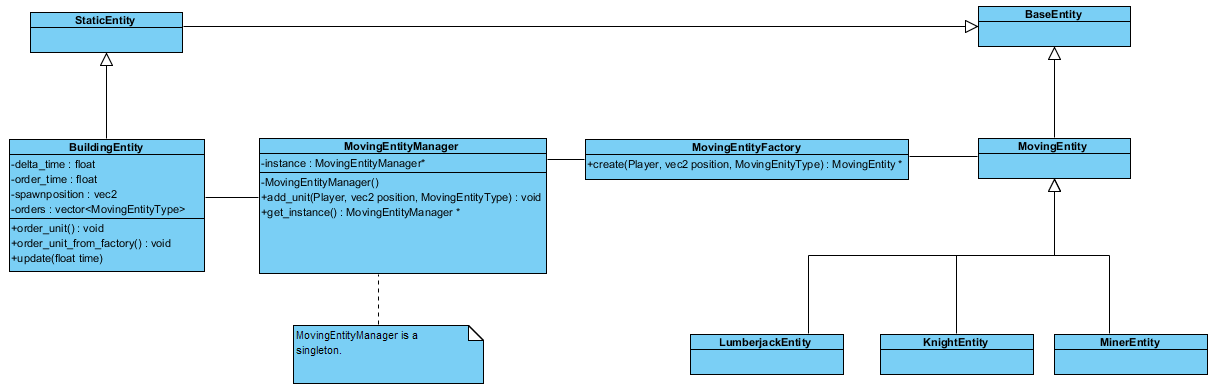
\includegraphics[scale=0.55]{res/MovingEntityFactoryClass.png}
    \caption{Class structure around the MovingEntity factory.}
\end{figure}
\newpage
 
There is also a rotated version of this image in the appendix for a sharper image if needed.

After the MovingEntityManager has completed an order from the factory the unit will spawn in the given location. This process will repeat until all orders have been handled.




